
\section{Conception et recherches}
\subsection{Planification}

\paragraph{Planification et partage des tâches}

La planification de notre projet a été structurée en quatre grandes phases : la recherche et la conception, la création du jeu, le développement des fonctionnalités en ligne, et la phase de finalisation. Le diagramme de Gantt ci-dessous illustre cette répartition temporelle et thématique. 

\begin{figure}[!h]
    \centering
    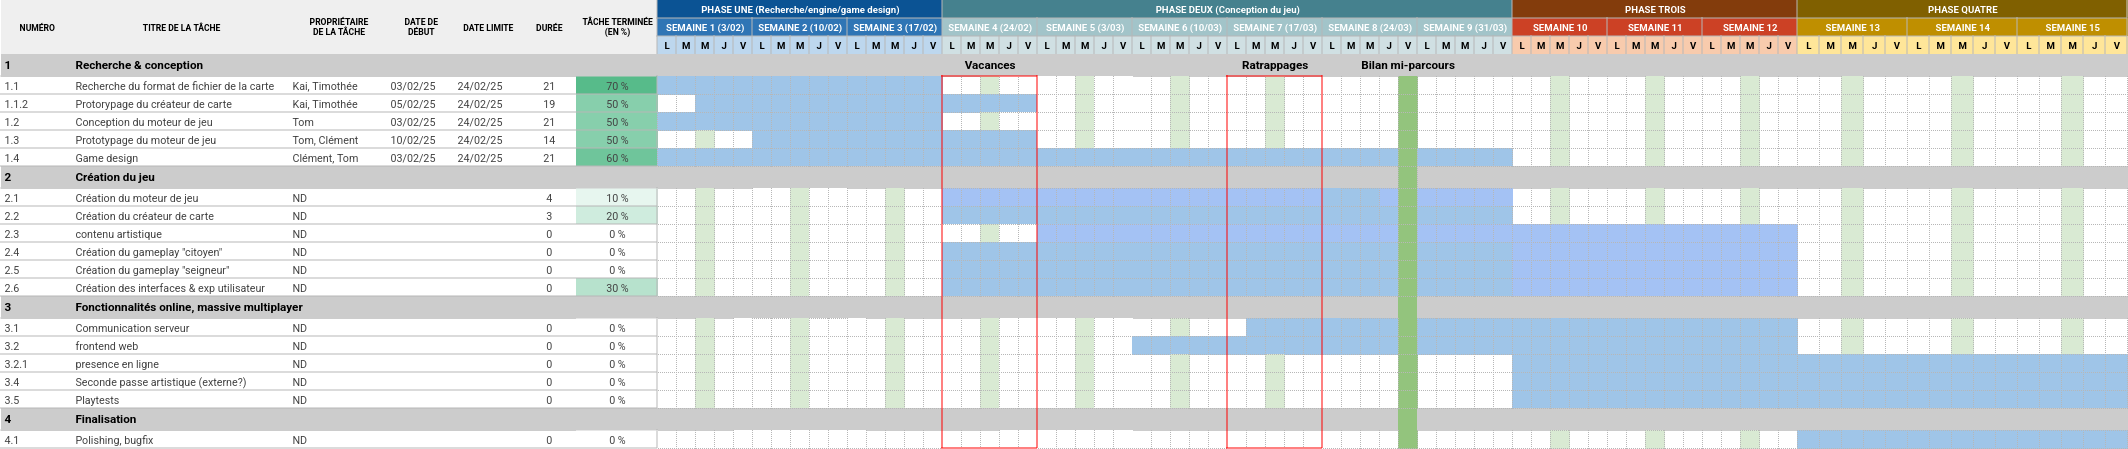
\includegraphics[width=0.99\linewidth]{images/gantt.png}
    \caption{Diagramme de Gantt}
    \label{fig:enter-label}
\end{figure}


Dès le début, nous avons identifié trois objectifs fondamentaux : développer un outil de génération de carte en C++, établir les bases du moteur de jeu en TypeScript (notamment à l’aide de la bibliothèque Three.js), et définir le design général du jeu. En conséquence, les tâches ont été réparties selon les affinités et compétences de chacun : Tom Zink a pris en charge le développement du moteur de jeu, Clément Saperes s’est concentré sur le game design, tandis que Kai Night et Timothée Bonetti ont collaboré sur l’outil de création de carte.

Les premières semaines ont été majoritairement dédiées à cette phase de recherche et de prototypage. Une fois ces bases posées, la deuxième phase du projet consistait à réunir les différents composants pour créer un gameplay cohérent (incluant les rôles « citoyen » et « seigneur »), concevoir les interfaces utilisateurs et assurer une interactivité fluide.


\paragraph{Imprévus}
Cependant, cette intégration s’est révélée plus complexe que prévu. Plusieurs obstacles ont freiné notre progression : une méconnaissance initiale de certaines technologies clés (notamment TypeScript et Three.js), le manque de bibliothèques satisfaisantes pour la création d'interfaces web, ainsi que des difficultés à coordonner notre travail en raison d’emplois du temps peu compatibles.

Ces contraintes ont nécessité une réévaluation continue de nos priorités et ont impacté l'avancement de certaines tâches, comme en témoigne le taux d’achèvement partiel de certaines activités dans le diagramme. Nous reviendrons plus en détail sur ces difficultés dans les sections suivantes de ce rapport.


